\subsection{Aristoteles}
Aristoteles (* 384 \ac{vCHR} in Stagira (Griechenland) – † 322 \ac{vCHR} in Chalkis) war Wissenschaftler, Biologe, Physiker und Philosoph. 

Als Sohn eines reiches Artzes war es ihm gegönt Platons Akademie zu besuchen. Er befasste sich zunächst mit mathematischen und dialekitschen Themen. Nach und nach begann er mit der Verfassung von eigenen Werken. Aristoteles blieb etwa 20 Jahre an der Akademie als Student und später als Lehrer. Nach dem Tod Platons verließ er Athen und seine sogenannten \glqq Reisejahre\grqq\ begannen. Während der Reisejahre ging Aristoteles auf Einladung von Philipp II. nach Mieza. Dort soll er den Sohn Alexander unterrichten. Dieser wird im Laufe der Geschichte zu Alexander der Große. Sein Weg führte ihn nun wieder nach Athen. Er forschte und lehrte an einem öffentlichen Gymnasium. Nachdem er sich von Alexander dem Großen und dem Königshaus abwandte, wurde ihm Gotteslästerung vorgeworfen. Daraufhin verließ er Athen und zog nach Chalkis. Dort starb er im Oktober 322 \ac{vCHR}. 

Aristoteles zählt bis heute noch zu den bekanntesten und einflussreichsten Philosophen und Naturforschern. Zu den berühmtesten Werken des Aristoteles zählen seine Poetik, Politik und Metaphysik.
\footnote{vgl. \url{https://de.wikipedia.org/wiki/Aristoteles}, abgerufen am 26.11.2017}\footnote{vgl. \url{https://www.geo.de/geolino/mensch/2755-rtkl-weltveraenderer-aristoteles}, abgerufen am 26.11.2017}

\begin{figure}[H]
\centering 
 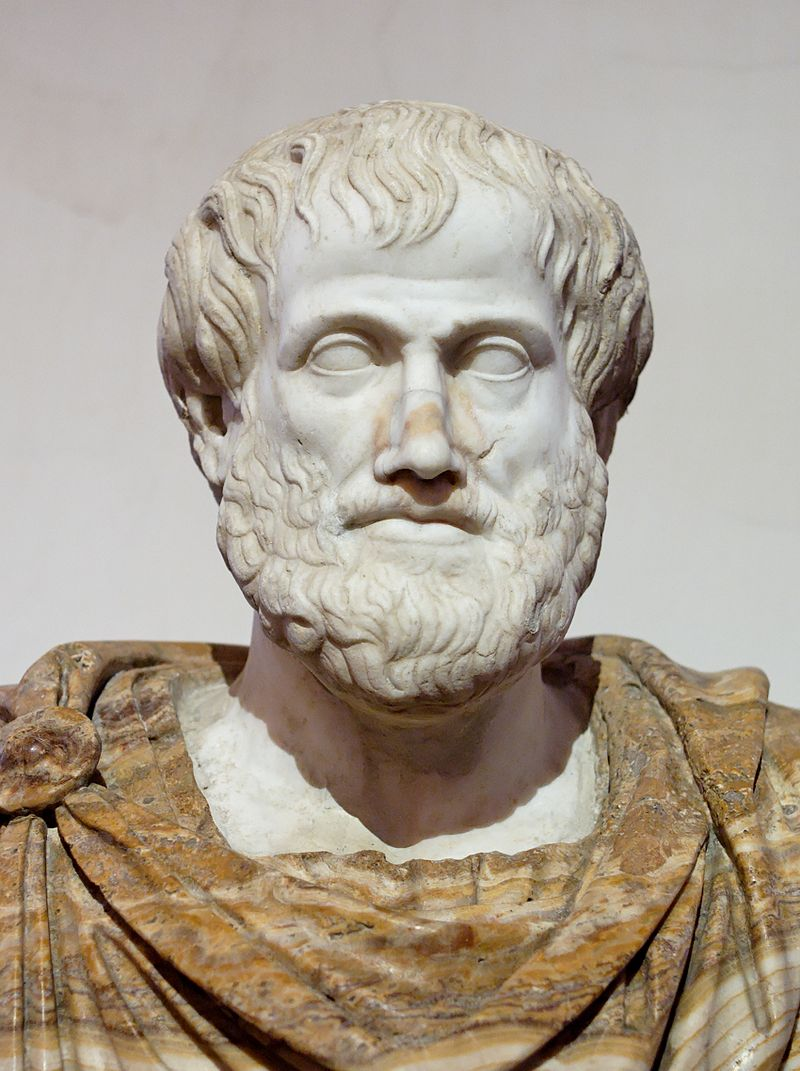
\includegraphics[width=0.3\textwidth]{Bilder/kap3/Aristoteles} 
 \caption{römische Kopie nach einer Skulptur des Bildhauers Lysippos \cite{WikiAR}  \label{portraitAristotles}}
\end{figure}

\subsubsection{Kernthesen}

An dieser Stelle werden die Thesen aus dem Dialog\footnote{In der ARD-Mediathek verfügbar unter der URL: \url{http://www.ardmediathek.de/tv/Denker-des-Abendlandes/Aristoteles/ARD-alpha/Video?bcastId=14913016&documentId=15666426}, abgerufen am 26.11.2017} zwischen Harald Lesch\footnote{Harald Lesch ist Physiker an der Ludwig-Maximilians-Universität München. Neben der Physik beschäftigt er sich mit der Philosophie.} und Wilhelm Vossenkuhl\footnote{Wilhelm Vossenkuhl ist ein emeritierter Professor für Philosophie an der Ludwig-Maximilians-Universität in München.} dargestellt werden. In diesem Dialog arbeiten die beiden bestimmte Thesen aus, die dann zur eigenen Meinungsfindung verwendet werden. Hiermit sei darauf hingewiesen, dass die folgenden Thesen nicht von den Autoren stammen.

Beginnen möchten wir die Ausarbeitung mit einer Aussage:
\paragraph{\glqq Aristoteles der erste große Logiker\grqq. } Er beschreibt die Logik als eine Art Handwerkszeug für die Lösung von Problemen. Welches Werkzeug aus meinem Werkzeugkoffer muss ich verwenden, um ein bestehendes Problem zu lösen. Aristoteles hat die Syllogistik (Logik) so weit entwickelt, dass für jede denkbare theoretische Situation ein Schlussverfahren möglich ist. Das Konzept besteht dabei aus Obersatz, Untersatz und Schluss.\footnote{Anmerkung seitens der Autoren, dieses Konzept kommt auch in der Rechtslehre zur Anwendung.} Harald Lesch nennt im Dialog dazu ein Beispiel: \glqq Wie komme ich (Harald Lesch) eigentlich zu irgendwelchen Schlüssen über Phänomene?\grqq. Lesch bezieht dies speziell auf die Astrophysik. Die Antwort liegt nahe, man verwendet die Logik um diese Phänomene handhabbar zu machen.

Nun folgen die Thesen:
\paragraph{Das natürliche Bestreben des Menschen ist zu Wissen}, diese These ist am Anfang der Metaphysik zu finden. Wissen ist etwas was neu werden kann, es erweitert sich.  

\paragraph{Alles geschieht wegen einem gewissen Zweck} Aristoteles war der Ansicht, dass alle Vorgänge im Leben zu einem gewissen Zweck passieren. Es gibt kein Handeln ohne einen gewissen Zweck. Die Sinnlosigkeit ist damit für Aristoteles ausgeschlossen.

\paragraph{Syllogistik bietet keine Antwort auf ethische Fragen} ist eine weitere These von Aristoteles. Somit ist klar, dass man ethische Fragen nicht mit wahr-falsch beantworten kann. Allgemein trennt Aristoteles die Methoden der Wissenschaft und Ethik. Für die Wissenschaft gibt es die Syllogistik. Bei der Ethik kommt die Fuzzylogik\footnote{Es gibt nicht nur die Werte null und eins. Zwischen  den Werten null und eins werden unendlich viele Werte eingeführt.} (Aussage Harald Lesch) ins Spiel.

\paragraph{Jedes Problem hat seine ihm eigene Genauigkeit} dies geht aus der Nikomachische Ethik des Aristoteles hervor. Das heißt einmal ist es gut genau hinzuschauen und einmal erweist es sich als besser weniger genau hinzuschauen. Kurz gesagt man soll nicht immer alles mit dem gleichen Maßstab messen.

\subsubsection{Chatbots zwischen Wissenschaft und Ethik}

Nun möchten wir die Aussagen und Thesen des Dialogs zu unserer eigenen Meinungsfindung verwenden. Ist es aus Sicht von Aristoteles vertretbar einen Chatbot zu verwenden? 

Aristoteles hat sich, wie eingangs erwähnt, vielen Gebieten gewidmet. Unter anderem auch der Wissenschaft. Er ist bekannt für seine Syllogistik. Eine abgewandelte Form dieser Syllogistik wird auch heute in Chatbots/\ac{ki} verwendet. Was wir heute Aussagenlogik nennen kommt der Vorstellung von Aristoteles am nächsten. Er trennt zwar die Wissenschaft mit ihrer Methode der Logik von der Ethik, allerdings spielt uns die Tatsache, dass Aristoteles sich mit der Logik beschäftigt hat in die Karten. Da die Logik ein Baustein der Chatbots/\ac{ki} ist wird Aristoteles nicht abgeneigt von der Idee eines Chatbots/\ac{ki} sein. 

Als nächstes soll folgende These bearbeitet werden, \glqq Jeder Mensch hat das Bestreben zu Wissen\grqq. Wir versetzen uns nun in die Lage eines Anwenders, der einen Support-Chatbot um Rat bittet. Aristoteles nennt in keiner Form wie die Übermittlung des Wissens stattfindet. Auch nennt er keine Quelle für das Wissen. Unser \glqq Problem\grqq\ ist es, dass das Wissen was der Mensch erfährt von einem Chatbot stammt. Wir sind der Meinung, dass der Chatbot/\ac{ki} als Wissensquelle in ein paar Jahren nicht mehr zur Debatte steht. Wissensquellen haben sich seit Anbeginn der Zeit verändert. Zuerst waren es die Gelehrten die das Wissen vermittelten. Oft nur durch mündliche Weitergabe. Denn der Rest der Bevölkerung konnte nicht lesen und somit aufgeschriebenes Wissen nicht konsumieren. Also oblag die Wissensweitergabe den Gelehrten. Mit dem Fortschreiten der Bildung unter der \glqq normalen\grqq\ Bevölkerung, war es auch für diese möglich niedergeschriebenes Wissen zu konsumieren. Nun kommen neben Gelehrten auch Aufzeichnungen (Bücher, etc.) als Wissensquelle ins Spiel. Die Menschen können sich nun unabhängig von den Gelehrten Wissen aneignen und weitergeben. Die Wissensquelle Aufzeichnungen steht heute für uns außer Frage. Nach den Bücher kommt für uns das Internet als Wissensquelle hinzu. Beim Internet als Wissensquelle kann man schon diskutieren. Aber wenn man weiß wie man das Internet als Wissensquelle zu verwenden hat, ist diese Wissensquelle genau so geeignet wie Bücher. Die Autoren stellen das Internet als Wissensquelle nicht in Frage. Wir sind der Überzeugung, dass dies auch mit den Chatbots/\ac{ki} als Wissensquelle im Laufe der Zeit passieren wird. Als Konklusion können wir sagen, dass ein Chatbot/\ac{ki} das Bestreben des Menschen nach Wissen nicht im Wege steht, eher sogar fordert.

\glqq Alles geschieht wegen einem gewissen Zweck\grqq. Der Chatbot erfüllt einen Zweck für das Unternehmen. Er soll zum Beispiel die Kunden beraten und bei Fragen zur Seite stehen. Ferner gesagt, soll er das Bestreben des Menschen zu wissen befriedigen. Ein Chatbot ist somit keineswegs von Sinnlosigkeit geprägt. Es besteht also kein Wiederspruch zur These.

Auch erkannte Aristoteles, dass ethische Fragen nicht pauschal mit wahr oder falsch beantwortet können. Daran hat sich auch heute noch nichts geändert. Wir sind heute noch in dem Dilemma ethische Fragen zum Wohle aller beteiligten zu beantworten. Harald Lesch nennt dazu das Beispiel der Fuzzylogik. Die Fuzzylogik zeichnet sich durch ihre Unschärfe in der Formulierung aus. Es kann nicht mehr auf wahr oder falsch geschlossen werden. Es ist irgendwas zwischen diesen Zuständen. Genau an dieses Problem gelangen wir, wenn wir ethische Fragen beantworten wollen.

\glqq Jedes Problem hat seine ihm eigene Genauigkeit\grqq. In unserem Fall ist es nicht getan das Thema nur kurz zu betrachten und dann eine Entscheidung zu treffen. So untersuchen wir in dieser Hausarbeit das Thema aus verschiedenen Blickwinkeln um dann eine passende Entscheidung zu treffen. Dies passt zur These, wir legen in diesem Fall eine hohe Genauigkeit an.

\paragraph{Abschließend} bleibt uns zu sagen, dass wir sehr erstaunt über die Einsichten von Aristoteles sind. Er erkannte schon zu seiner Zeit, dass für verschiedene Disziplinen wie Wissenschaft oder Ethik verschiedene Werkzeuge nötig sind. Seine strikte Trennung von Wissenschaft und Ethik ist heute noch gültig. Auf der Grundlage der bisher diskutierten Gedanken sehen wir keine Handhabe die gegen die Verwendung von Chatbots sprechen. 

